\documentclass[a4paper,oneside,onecolumn]{article}
\usepackage[utf8x]{inputenc}
\usepackage[T1]{fontenc}
\usepackage{lmodern}
\usepackage{mathtools}
\usepackage{color}
\usepackage{siunitx}
\usepackage{microtype}
\usepackage{fancyhdr}
\usepackage{amsmath}
\usepackage{listings}
\usepackage{amssymb}
\usepackage{}
\usepackage[head=12pt,hmargin=2.5cm,vmargin=2.5cm]{geometry}

\renewcommand*\lstlistingname{Code Snippet}

\definecolor{codegreen}{rgb}{0,0.6,0}
\definecolor{codegray}{rgb}{0.5,0.5,0.5}
\definecolor{codepurple}{rgb}{0.58,0,0.82}
\definecolor{backcolour}{rgb}{0.95,0.95,0.92}

\lstdefinestyle{mystyle}{
    backgroundcolor=\color{backcolour},   
    commentstyle=\color{codegreen},
    keywordstyle=\color{magenta},
    numberstyle=\tiny\color{codegray},
    stringstyle=\color{codepurple},
    basicstyle=\footnotesize,
    breakatwhitespace=false,         
    breaklines=true,                 
    captionpos=b,                    
    keepspaces=true,                 
    numbers=left,                    
    numbersep=5pt,                  
    showspaces=false,                
    showstringspaces=false,
    showtabs=false,                  
    tabsize=2
}
 
\lstset{style=mystyle}

\DisableLigatures[>,<]{encoding = T1,family=tt*} %

\definecolor{codegray}{gray}{0.9}
\newcommand{\code}[1]{\colorbox{codegray}{\texttt{#1}}}

\pagestyle{fancy}

\begin{document}

\title{Lab 4 \\ Kernel Patching and Cross-Compilation for RPi \\ Embedded Linux}
\author{Julia Desmazes \\ Michael Nissen}
\date{\today}
\maketitle
\bigskip

\section{Download / Set the good version of Linux sources}

\noindent
To execute the tasks for this report, the first step is to get the Raspberry Pi cross-compilation tools, and specific version of the linux kernal that one wants to patch. This is going to be done using \code{git clone}, which ofcourse assumes a working installation of \texttt{git}.
\newline
To get the latest version of the kernel source code and the cross-compilation tools, the following commands with be copied to the terminal:
\begin{lstlisting}
host$ git clone https://github.com/raspberrypi/tools.git
host$ git cone -b rpi-4.4.y https://github.com/raspberrypi/linux.git
\end{lstlisting}
One now has to make sure to get the same configuration as is used by ones Raspberry Pi during the kernel compilation, which can be done by checking out the \texttt{git branch} that corresponds to the hash of the Linux kernel running on the Raspberry Pi.
\newline
This will be done by by running the shells script seen in Code Snippet \ref{lst:git_hash}. This shell script will grep the firmware hash found on the Raspberry pi, and then get the \texttt{git hash} from the github link relative to the hardware hash.
\begin{lstlisting}[caption={Shell script to get Linux kernel git hash}, label={lst:git_hash}]
#!/bin/bash

PLATFORM=`uname -s` 

if [ ${PLATFORM} = "Darwin" ]
then
    CMD="gunzip -c"
elif [ ${PLATFORM} = "Linux" ]
then
    CMD="zcat"
else
    echo "Sorry, the platform ${PLATFORM} is not supported !!!"    
    exit -1
fi

FWHASH=`${CMD} /usr/share/doc/raspberrypi-bootloader/changelog.Debian.gz | grep -m 1 'as of' | awk '{print $NF}'`
#echo "Firmware Hashcode: fwhash = $FWHASH"

LINUXHASH=`wget -qO- https://raw.github.com/raspberrypi/firmware/$FWHASH/extra/git_hash`

echo "Linux Hashcode: linuxhash = $LINUXHASH"
\end{lstlisting}
When one has figured out the \texttt{git hash}, one can change directory to the linux git repository and checkout the respective brach by the following command:
\begin{lstlisting}
host$ cd linux
host$ git checkout <git_hash>
host$ make clean -mrproper
\end{lstlisting}
At line 3, we are cleaning kernel tree from all unneeded files of the first version which is a recommended practice prior to each kernel compilation!

\section{Patch the Kernel}
Before starting to patch the kernel, one should make sure to identify the Linux sources that one is trying to install. This can be done using the \code{head} command, which will look like this:
\begin{lstlisting}
host$ head Makefile

	# Ouput generated by running head on the Makefile #
	VERSION = 4
	PATCHLEVEL = 4
	SUBLEVEL = 21
	EXTRAVERSION = 
	NAME = Blurry Fish Butt
\end{lstlisting}
Now that one know the specific version of the Linux kernel, it is time to download the latest \texttt{PREMEPT-RT} patch that corresponds to ones kernel version - if follows the format: \texttt{version.patch-level.sub-level}.
\newline
To download the patch from the patch from \texttt{kernel.org} using the \code{wget} command like so: 
\newline
\code{wget https://cd.kernel.org/pub/linux/kernel/projects/rt/4.9/patch-4.9.47-rt47.patch.gz}
\newline
\newline
Now one can actually start patching the kernel sources by executing the following commands in succession:
\begin{lstlisting}
host$ gunzip patch-<version.patch-level.sub-level>-rt<last>.patch.gz
host$ cat patch-<version.patch-level.sub-level>-rt<last>.patch | patch -p1
\end{lstlisting}
One can now create a folder named \texttt{rt-modules} under your project folder - at the same level as the \texttt{linux} and \texttt{tools} folders, and export an environment variable \texttt{INSTALL\_MOD\_PATH} that points to that folder:
\begin{lstlisting}
host$ mkdir rt-modules
host$ cd rt-modules
host$ export INTALL_MOD_PATH=$PWD
\end{lstlisting}
Here \code{\$PWD} is the path to the current directory.

\section{Configure Cross-compilation}

Before starting the cross-compilation, one is going to specify the architecture for which to compile, the cross-compiler that ones wishes to use, and the kernel that one is trying to compile for. This is done by exporting some specific environment variables that is used by the makefile:
\begin{lstlisting}
host$ export ARCH=arm KERNEL=kernel7
host$ export CROSS_COMPILE=$PWD/tools/arm-bcm2708/gcc-linaro-arm-linux-gnueabihf-raspbian-x64/arm-linux-gnueaihf-
\end{lstlisting}
Now, to configure the kernel in an appropriate way, one can use the existing kernel configuration from the Raspberry Pi. This configuration file can be generatied using the \code{modprobe} command, and then copy that generated file from the Raspberry Py over to the \texttt{linux/} folder on the host machine using the \code{scp} command. Finaly, extract the content of the \texttt{config.gz} into a \texttt{.config} file:
\begin{lstlisting}
host$ sudo modprobe configs
host$ scp pi@193.169.0.26:/proc/config.gz /home/user/kernel_labs/linux
host$ zcat -c config.gz > .config
\end{lstlisting}
Now that one has created a default \texttt{.config} file, it is time to costumise the kernel using the \code{sudo make menuconfig} which opens the GUI seen in Figure \ref{fig:menuconfig}. For the purpose of this lab assignment, we are going to enable the \texttt{Fully Preemptible Kernel} setting, and the \texttt{High Resolution Timer Support}.
\begin{figure}[htbp]
	\centering
	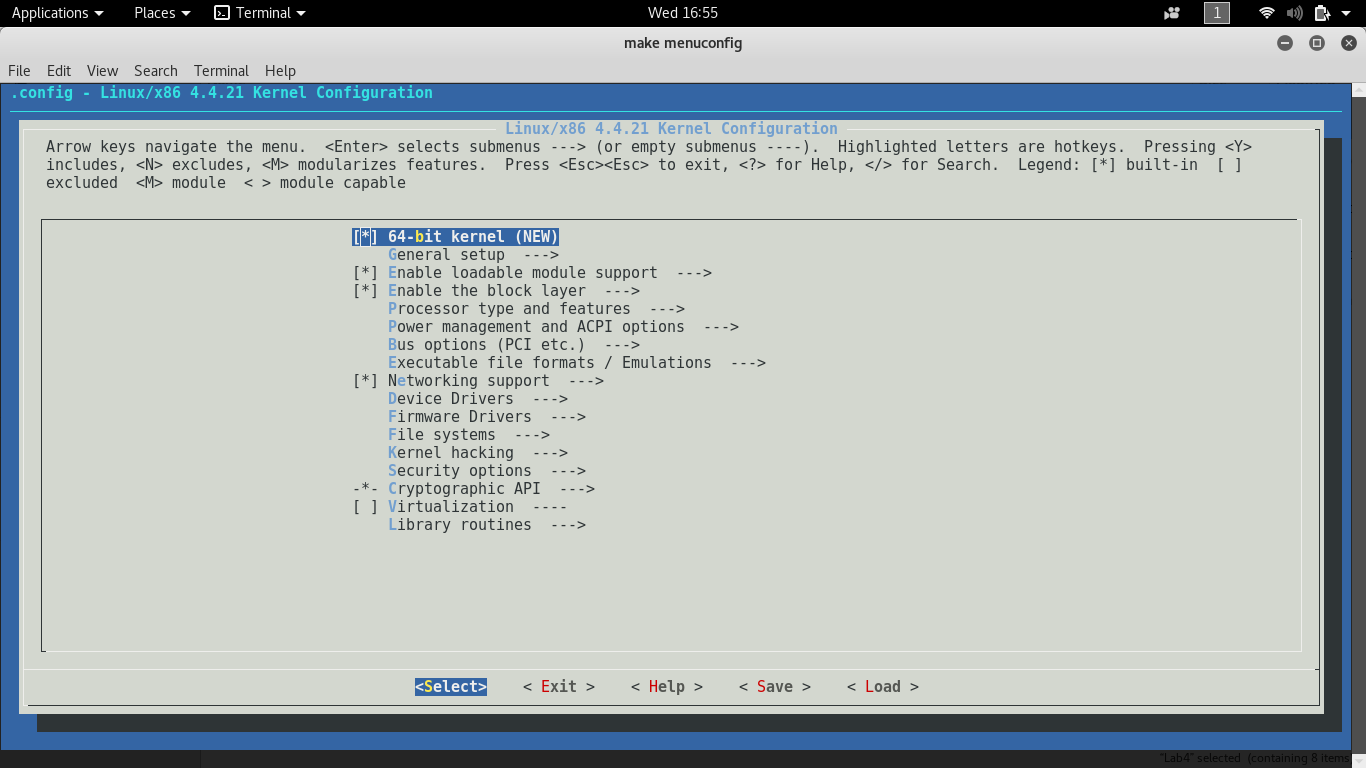
\includegraphics[width=0.95\textwidth]{resources/meunconfig.png}
	\caption{caption}
	\label{fig:label}
\end{figure}

\newpage
\section{Build the new Kernel and Modules}

To build the kernel,and modules we have to compile our configured sources before they can be run by our pi.  This is where all of our exported variables comme into play, they will be used in the compilation processe to assurw we are doing a cross compilation.\newline
Once we know the number of availible CPU's by using the \code{nproc}, we need to build the kernel with it's file system and the modules.
\begin{lstlisting}
host$ make -j < 2* number of CPU > zImage modules dtbs
\end{lstlisting}
Once the modules are compiled we can install them to the path scpecified by \code{\$INSTALL MOD PATH}.
\begin{lstlisting}
host$ make -j < 2* number of CPU > modules_intall
\end{lstlisting}
Our next step is to create is to replace bootable kernel image based with the ones in our compiled sources. We created this image with zImage but it still needs some post-processing to support the dtbs type file system. To do theys changes we use \code{mkknling} a small utilitay found in tools that essentially justs adds \texttt{boot-uncompressed.txt} and \texttt{args-uncompressed.txt} to our image and creats a new image named kernel7.img in our recently created directory \texttt{\\boot}.
\begin{lstlisting}
host$ mkdir $INSTALL_MOD_PATH/boot/
host$ ./scripts/mkknlimg ./arch/arm/boot/zImage $INSTALL_MOD_PATH/boot/$KERNEL.img
\end{lstlisting}
We also need to add our \code{.dtb} files, theys files are essentially a database that represents the hardware components on out pi, so they to will be necessary at boot. We also copy in the overlays folder.
\begin{lstlisting}
host$ cp ./arch/arm/boot/dts/*.dtb $INSTALL_MOD_PATH/boot/
host$ cp -r ./arch/arm/boot/dts/overlays $INSTALL_MOD_PATH/boot
\end{lstlisting}
Now we should have a \texttt{boot} and an \texttt{lib} folder under our file location \texttt{\$INSTALL MOD PATH}. We can now transfert it to our pi for merging and to make the transfert faster we will first create a archive of our directory.
\begin{lstlisting}
host$ tar -cvzf kernel.tgz $INSTALL_MOD_PATH/*
host$ scp kernel.tgz pi@<IP adresse>:/tmp
host$ ssh pi@<IP adresse>
pi$ tar -zcvf /tmp/kernel.rgz /tmp/
\end{lstlisting}
Now we can start merging with the existing kernel on the pi, this processe is very simple, it envoloves coping recursively our files from boot and lib into the pi's own boot and lib folders.
\begin{lstlisting}
pi$ rm -rd /tmp/boot/overlays
host$ cp -rd /tmp/boot/* /boot/
host$ cp -rd /tmp/lib/* /lib/
\end{lstlisting}
At the end of the process we deactivate an option in our kernel for fast sd card interaction as it may cause problemes further on in our realtime kernel. Afterwars we can reboot and should have a realtime preemptive kernel.\newline
\begin{lstlisting}
pi$sudo nano /boot/cmdline.txt 

	# add sdhci_bcm2708.enable_llm=0 at the end of the line

pi$ sudo reboot now
\end{lstlisting}

\section{Preemptible kernel check}
To check if the new kernel is preemptive we check for two flags, the first is if the kernel type is said to be preemptive, this is the output we would get with \code{uname -a}. The second flag is located in file \code{/sys/kernel/realtime} if the file existis and if it's conents is 1 then we know the kernel is preemptive.
\begin{lstlisting}
host$ scp iffprempt.c pi@<IP address>:~/
host$ ssh pi@<IP address>
pi$ gcc -o iffpreempt ifpreempt.c
pi$ chmod +x iffreempt
pi$ ./iffreempt
this is a PREEMPT RT kernel
\end{lstlisting}
\section{Select the scheduling policy}
The \code{chrt} command allows us to run a process with a specific scheduling policy and priority ( when availible), it also allows us to see what availible options there are. If we wanted to lauch a preemptive processe we would use option \code{-r} and \code{-p} to define it's priority.\newline
If we wanted to lauch a SCHED\_FIFO process we would use the same commande but with oprion \code{-f} this time to specify FIFO.
\begin{lstlisting}
pi$ chrt -m

	# Output generated by running the above command
	SCHED_OTHER min/max priority	: 0/0
	SCHED_FIFO min/max priority	: 1/99
	SCHED_RR min/max priority	: 1/99
	SCHED_BATCH min/max priority	: 0/0
	SCHED_IDLE min/max priority	: 0/0

pi$ chrt -r -p <priority from 1/99> <process name> <args>
pi$ chrt -f -p <priority from 1/99> <process name> <args>
\end{lstlisting}

\section{Boot time optimization}

One thing we can notice is how slow the pi's boot is, according to \code{systemd-analyze time} the boot sequence takes un an entire 33.927 seconds, 31.531 of thoses for userspace. In otherwords there are more than 31 seconds of the boot sequence on witch we can have an effect. What is intresting is that when we go more into detail we realise that the dhcpcd services use up an entire 16.374 seconds.
\begin{figure}[htbp]
	\centering
	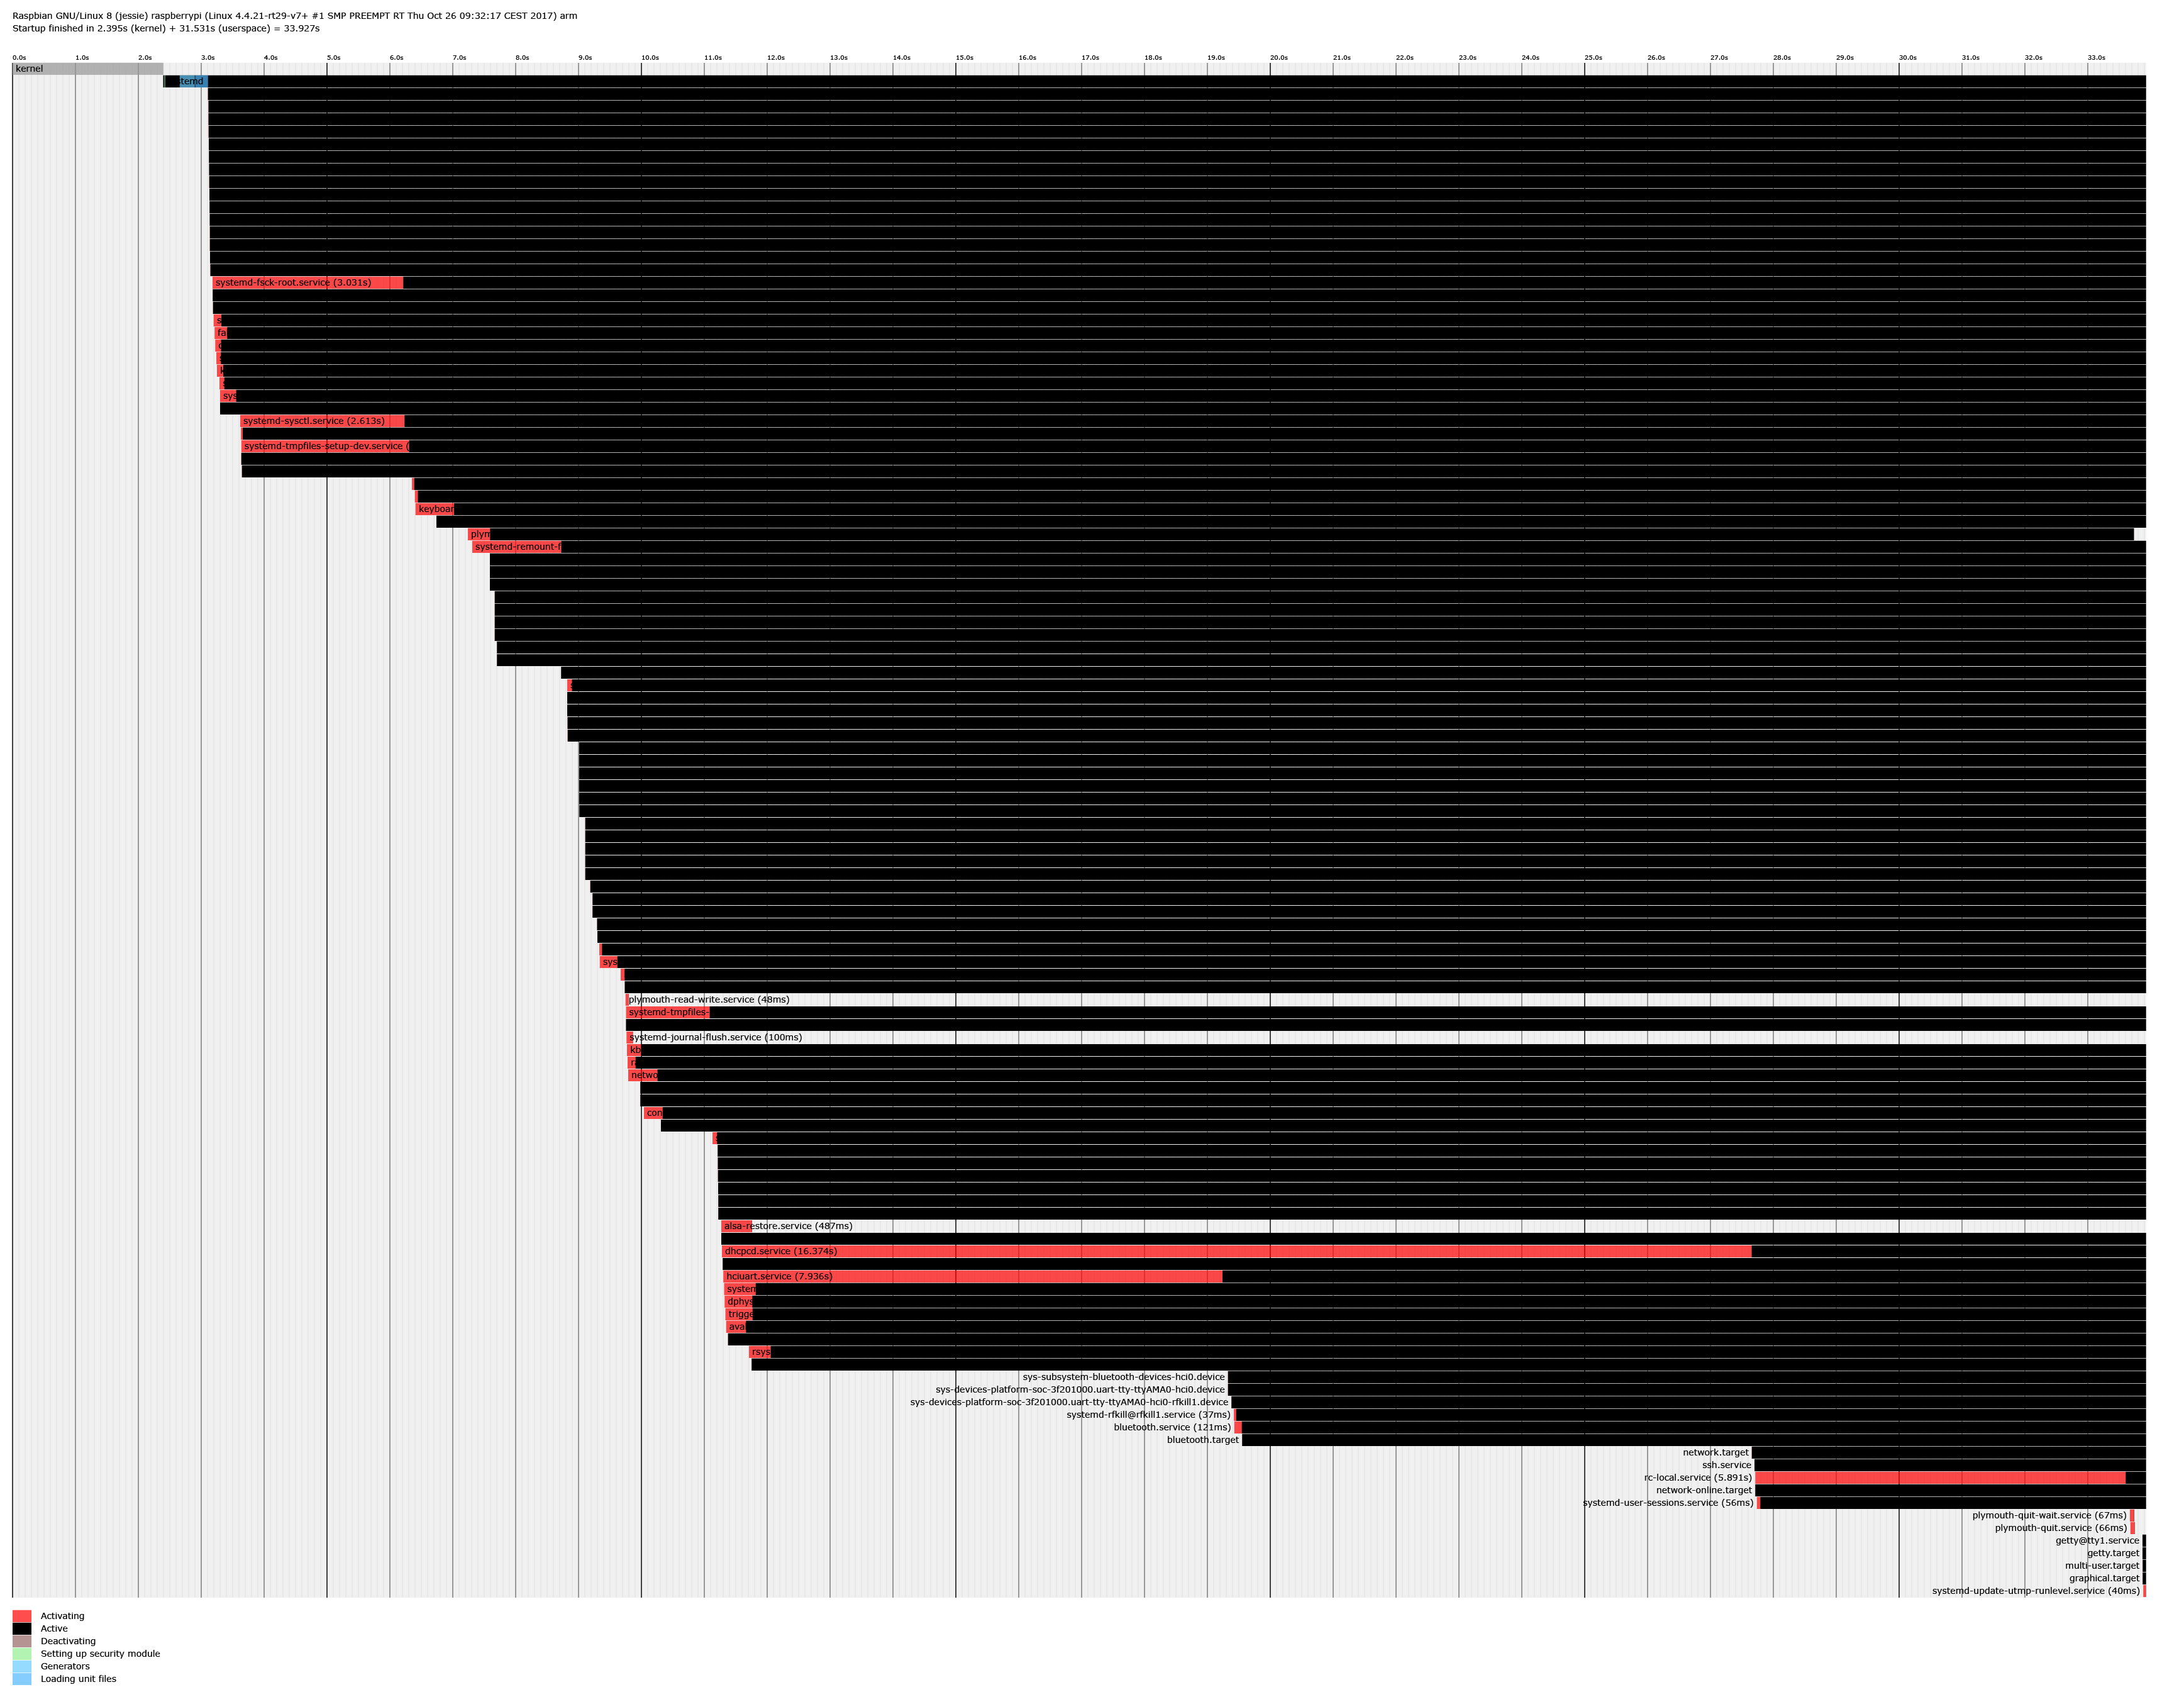
\includegraphics[width=0.95\textwidth]{resources/bootdyn.png}
	\caption{Boot sequence with dynamic ip}
	\label{fig:label}
\end{figure}
To reduce this time it was decided that sinc dhcp services are responable ( amoungs many other talsks ) for managing dynamic ip attributions, a way to speed it up would be to set un a static ip.\newline
To do this we included our static network configurations into \code{/etc/dhcpcd.config}.
\begin{lstlisting}
	# the interface we are currently using
interface eth0
	# our current ip address
static ip_address=192.168.1.79/24
	# my home rooters ip address
static routers=192.168.1.1
	# google's dns server adress
static domain_name_servers=8.8.8.8.8.8.4.4
\end{lstlisting}
We didn't configure wlan0 because, in case this failed we would have to manually alter the config files from the sd card.\newline
After reboot, we re-tested our boot time and it had significanly got shorter down to 20.993 seconds and 18.684 for userspace. Our dhcp service now only used up 6.907 seconds of boot time. If we wanted to ge further we could start dissabling services like bluetooth or hciuart that take up boot time and that we currently have no use for.
\begin{figure}[htbp]
	\centering
	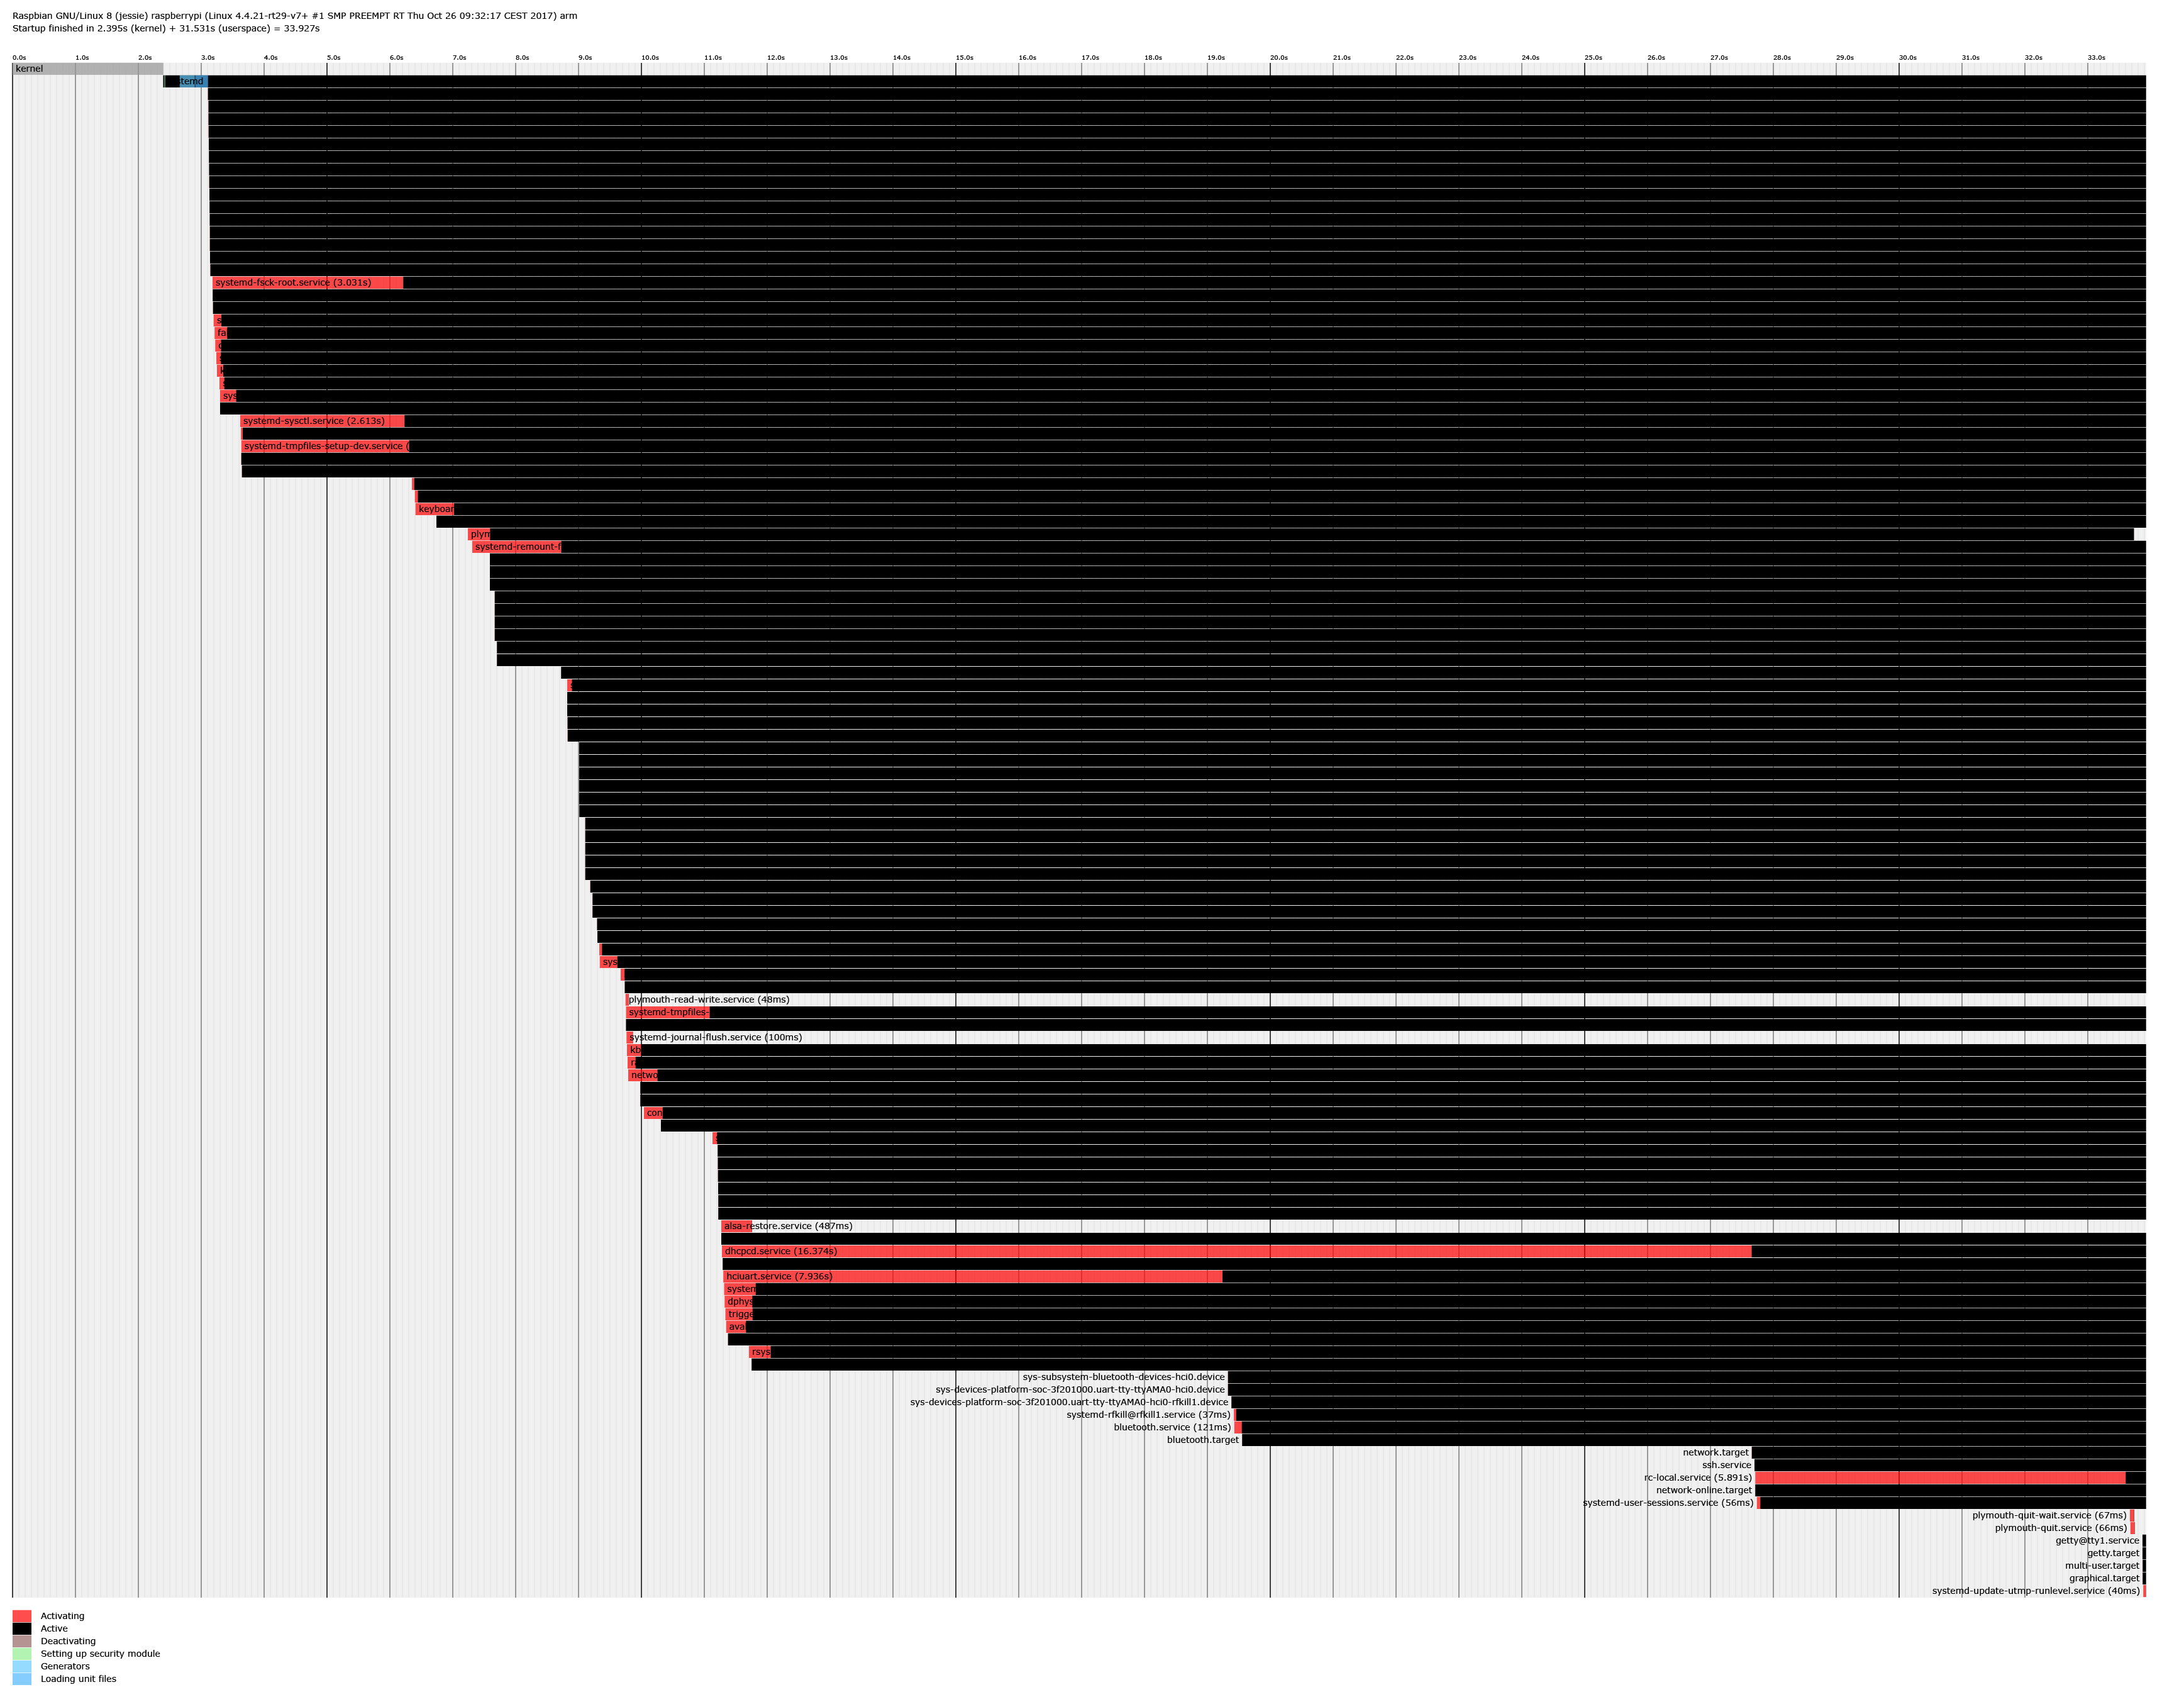
\includegraphics[width=0.95\textwidth]{resources/bootdyn.png}
	\caption{Boot sequence with dynamic ip}
	\label{fig:label}
\end{figure}

\section{Kernel modules}

\subsection{Create and compiling modules}

Code for hello.c:
\begin{lstlisting}
#include <linux/module.h>       
#include <linux/kernel.h>  
#include <linux/init.h>   

MODULE_AUTHOR("Julia Desmazes");
MODULE_LICENSE("GPLv3");
MODULE_DESCRIPTION("A short and winey hello world");

static int __init hello_hummans(void) {

	printk(KERN_INFO"Loading hello module...\n");
	printk(KERN_INFO"Hello world I am a module and I am loaded, chears and cookies \n");

	return 0;
}

static void __exit hello_end(void) {

	printk(KERN_INFO "Goodbye cruel world, oh why don't you love me?\n");
	printk(KERN_INFO"Module has been murdered...\n");
}

module_init(hello_hummans);
module_exit(hello_end);
\end{lstlisting}
Accompaning makefile:
\begin{lstlisting}
obj-m += hello.o
all:
	make ARCH=$(ARCH) CROSS_COMPILE=$(CROSS_COMPILE) -C $(DIR_TO_KERNEL) M=$(PWD) modules

clean:
	make -C $(DIR_TO_KERNEL) M=$(PWD) clean
\end{lstlisting}
We hade to perform a few changes to our environmental bash variables , first we changed the value of CROSS\_COMPILE to account for the fact that we here compiling form folder \texttt{extra}. Then we created \code{DIR TO KERNEL} that is the absolute path to our kernel compilation.
\begin{lstlisting}
#done from extre
export CROSS_COMPILE=$PWD/../tools/arm-bcm2708/arm-bcm2708-linux-gnueabi/bin/arm-bcm2708-linux-gnueabi-
export DIR_TO_KERNEL=$PWD/../linux/
\end{lstlisting}

\subsection{Loading/Unloading modules}

After having copied the modules to the pi with the \code{scp} protocol we then use \code{sudo insmod hello.ko} to load the module. We then checked to see if the module had been loaded by printing out a list of all the loaded modules with \code{lsmod | less}. Then to unload it we would use \code{sudo rmmod hello}.
\begin{lstlisting}
Module                  Size  Used by
hello                    944  0 
bnep                   10668  2 
hci_uart               19492  1 
btbcm                   6245  1 hci_uart
bluetooth             338111  22 bnep,btbcm,hci_uart
\end{lstlisting}
So we know our module was loaded but we were not getting any messages, we supposed this came from the fact that we where in as root under run level 3. To be shure the messages there we checked with \code{dmesg}.
\begin{lstlisting}
[ 7236.713120] Loading hello module...
[ 7236.713133] Hello world I am a module and I am loaded, chears and cookies 
[ 7345.372593] Goodbye cruel world, oh why don't you love me?
[ 7345.372616] Module has been murdered...
\end{lstlisting}
And, we confirmed our module was unloaded:
\begin{lstlisting}
odule                  Size  Used by
bnep                   10668  2 
hci_uart               19492  1 
btbcm                   6245  1 hci_uart
bluetooth             338111  22 bnep,btbcm,hci_uart
\end{lstlisting}
\end{document}